\section{Appendix}

\subsection{Tests with other meta-parameters}

Features and their statistics are given in the tables A.1 and A.2. An overlap can be seen but due to the different modelling in 4FGL there is a difference in the features.
%\dima{The description here is too short, in particular Figures A.1 and A.2 are not mentioned. Also the next appendix is very short. I think we can join the two appendices and call it something like ``Further tests of metaparameters''.}

\vspace{1cm}

\pgfplotstableread[col sep=comma]{data/features/3fglassocfeatures.csv}\tablea
\begin{table}
\resizebox{0.45\textwidth}{!}{
\pgfplotstabletypeset[
columns={Name,Mean,SD,Minimum,Maximum},
column type=c,
string type,
every head row/.style={before row=\toprule,after row=\midrule,},
every last row/.append style={after row={\hline} },
every first column/.style={column type/.add={|}{}},
every last column/.style={column type/.add={}{|}},
columns/Name/.style={column name=Feature Name,string replace*={_}{\textunderscore}},
columns/Mean/.style={column name=Mean,column type=c,numeric type,fixed,precision=2},
columns/SD/.style={column name=Standard Deviation,numeric type,fixed,precision=2},
columns/Minimum/.style={column name=Minimum,numeric type,fixed,precision=2},
columns/Maximum/.style={column name=Maximum,numeric type,fixed,precision=2},
skip rows between index={10}{25}
]{\tablea}
}
\vspace{0.2cm}
\caption{Statistics of features from the 3FGL which were used}
\end{table}

\pgfplotstableread[col sep=comma]{data/features/4fglassocfeatures.csv}\tableaf
\begin{table}
\resizebox{0.45\textwidth}{!}{
\pgfplotstabletypeset[
columns={Name,Mean,SD,Minimum,Maximum},
column type=c,
string type,
every head row/.style={before row=\toprule,after row=\midrule,},
every last row/.append style={after row={\hline} },
every first column/.style={column type/.add={|}{}},
every last column/.style={column type/.add={}{|}},
columns/Name/.style={column name=Feature Name,string replace*={_}{\textunderscore}},
columns/Mean/.style={column name=Mean,column type=c,numeric type,fixed,precision=2},
columns/SD/.style={column name=Standard Deviation,numeric type,fixed,precision=2},
columns/Minimum/.style={column name=Minimum,numeric type,fixed,precision=2},
columns/Maximum/.style={column name=Maximum,numeric type,fixed,precision=2},
%skip rows between index={17}{28}
]{\tableaf}
}
\vspace{0.2cm}
\caption{Statistics for finalized features from 4FGL }
\end{table}


Amongst all the algorithms, there exist certain hyper-parameters which haven't been discussed before. This was due to the fact that the impact of these hyper-parameters was not significant enough. For instance, logistic regression has two hyper-paramteres called regularization and tolererance. These features are the limit up to which one wants to go before accepting a solution. 
\begin{figure}[h]
%\centerin
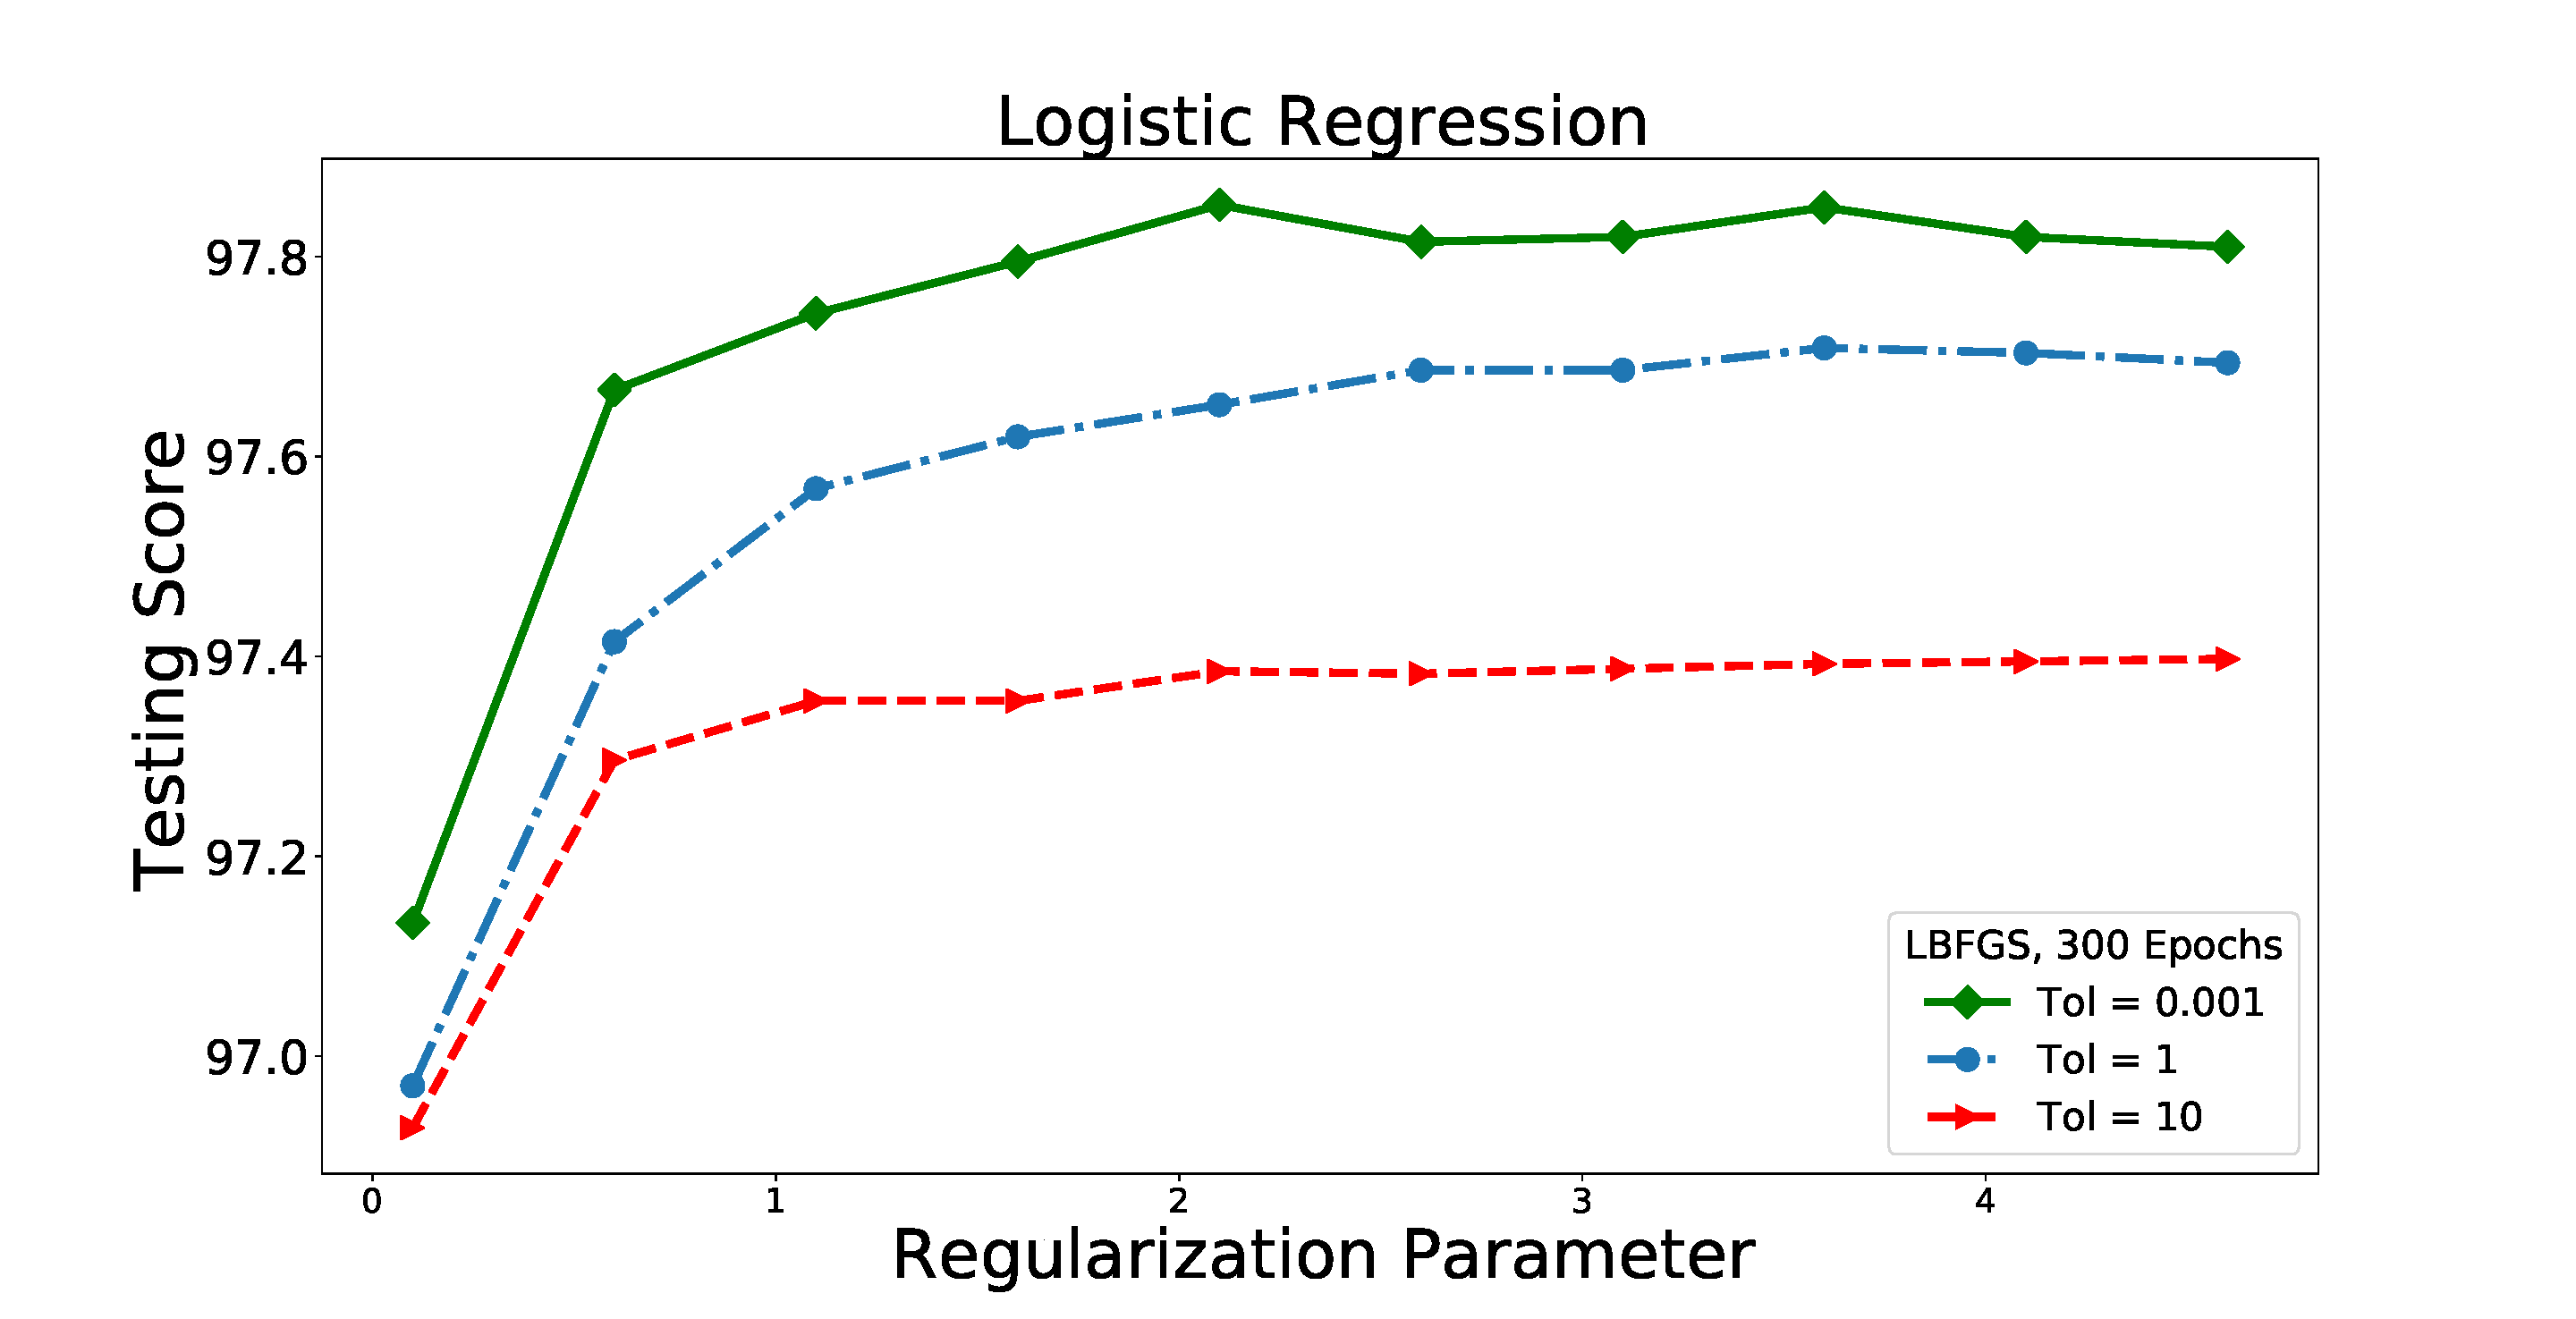
\includegraphics[width=\twopicsp\textwidth]{plots/lr_train_reg.pdf}
%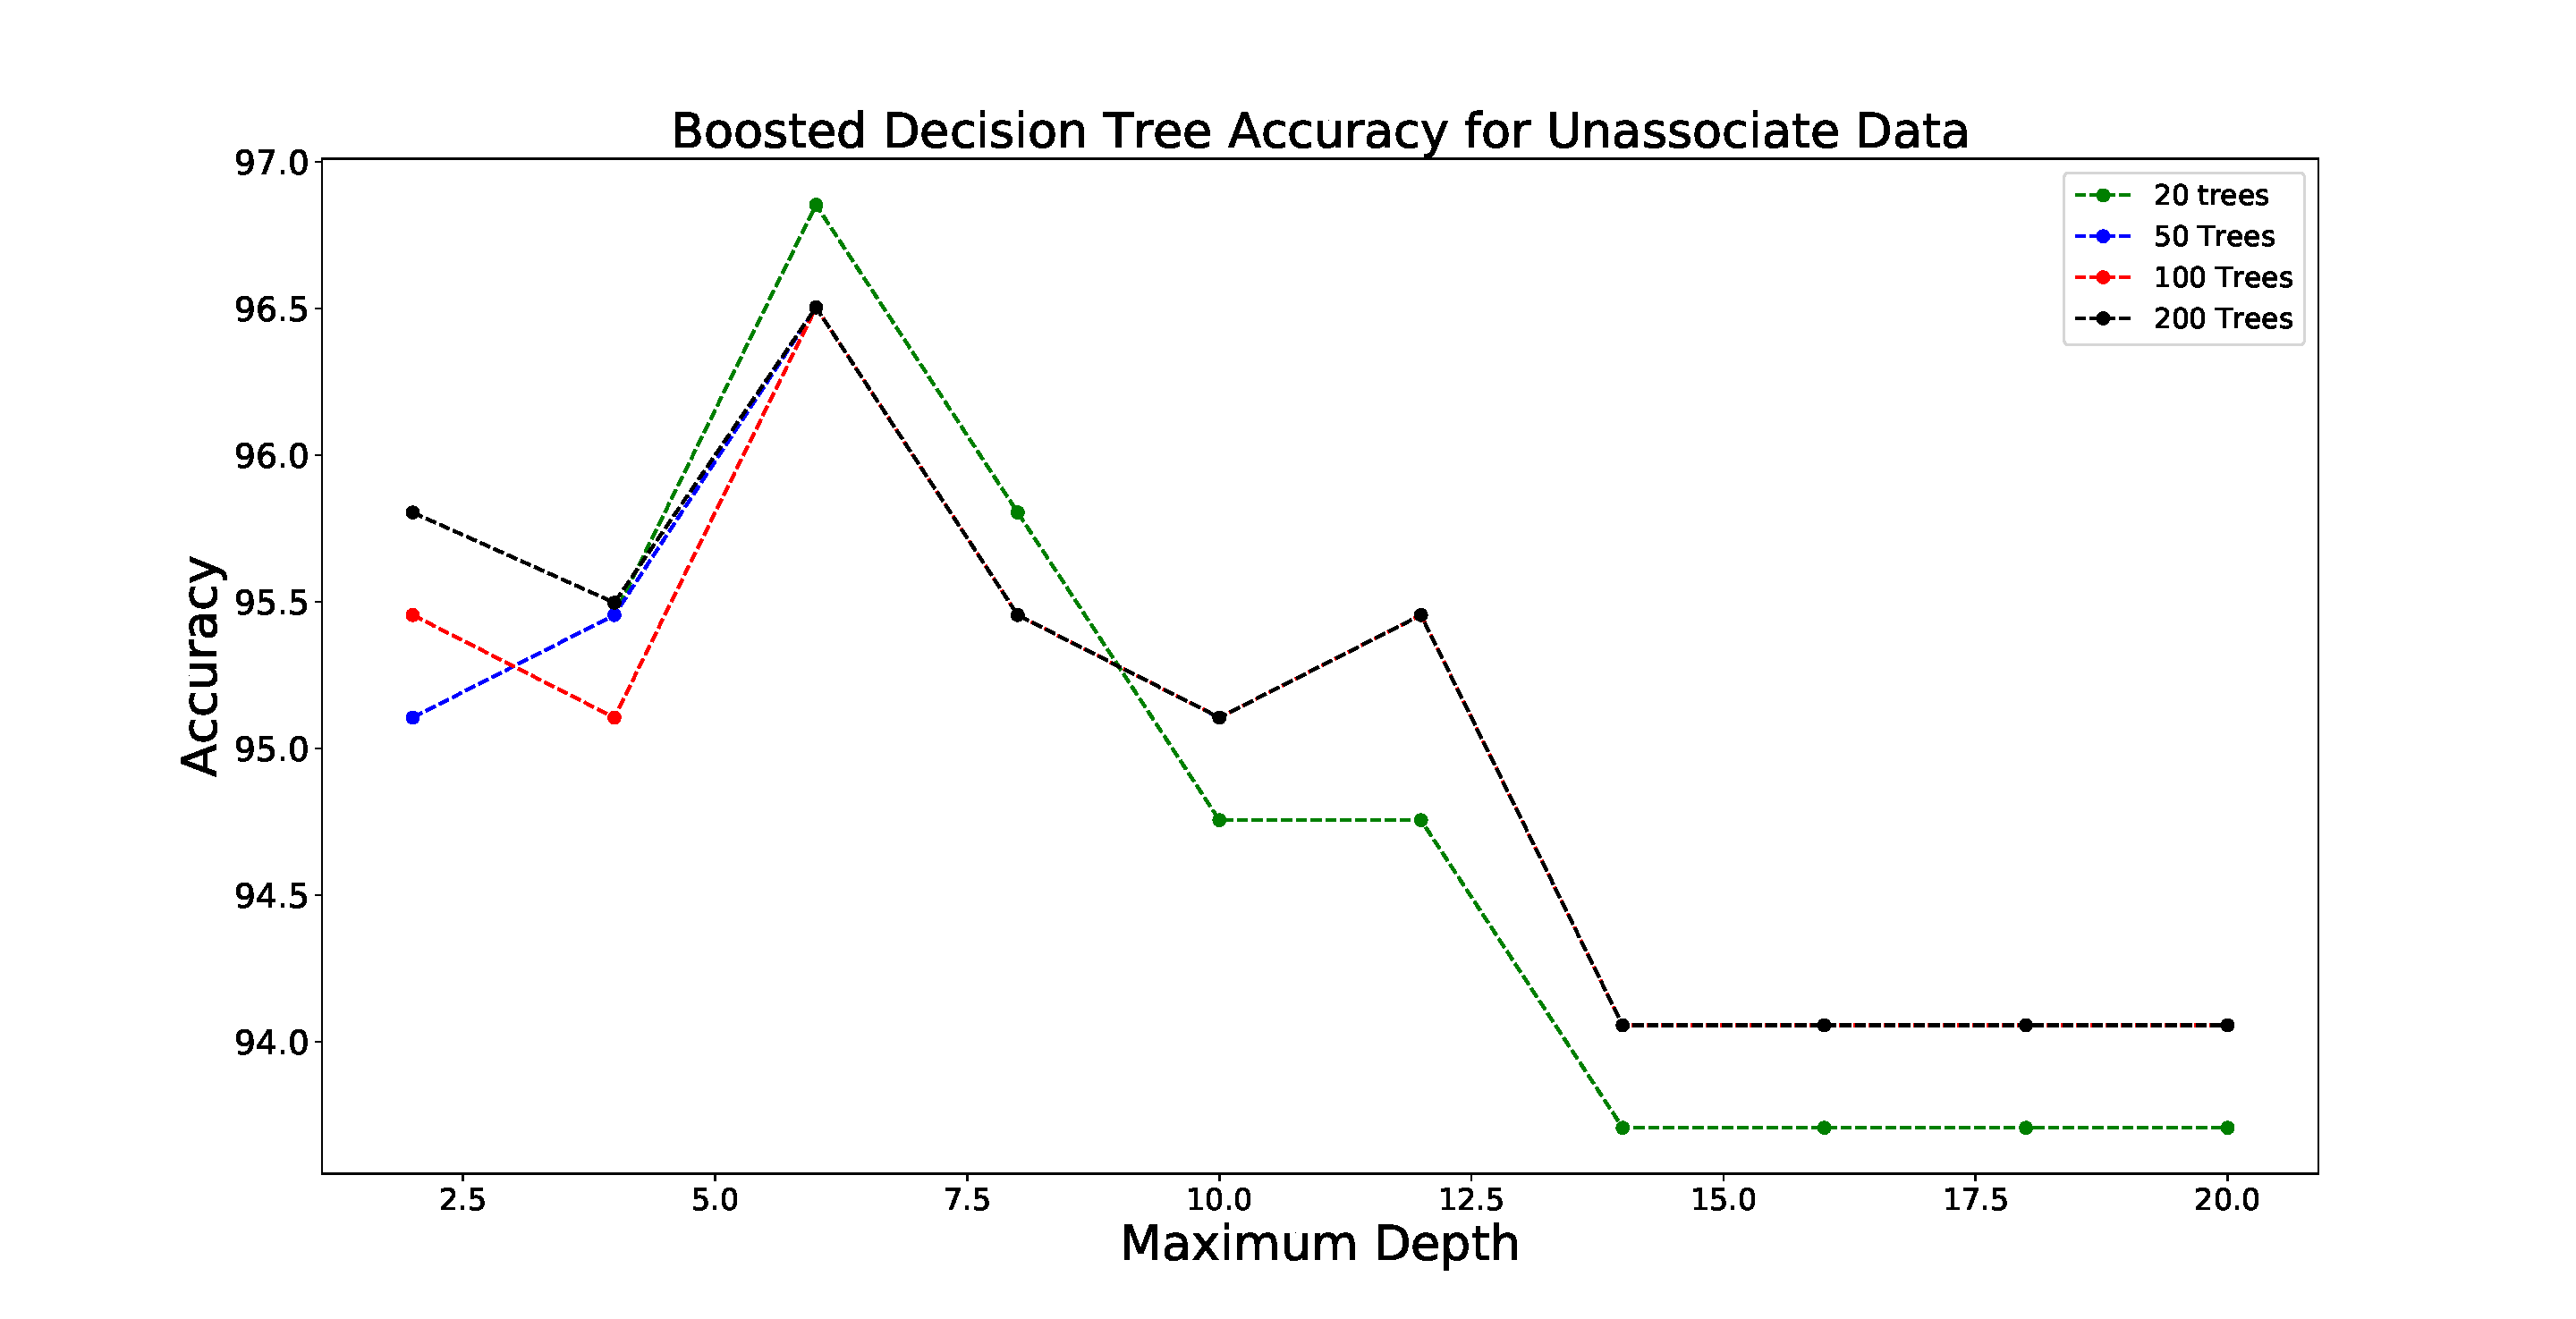
\includegraphics[width=\twopicsp\textwidth]{plots/unassoc_complex.pdf}
\caption{Dependence of LR on tolerance and regularization}
\label{fig:Lr_tol_reg}
\end{figure}
As can be seen in figure \ref{fig:Lr_tol_reg} the effect is not as significant as one would expect, and therefore only the default value of the two was considered. A similar effect is seen with neural networks in figure \ref{fig:nn_nn}, where increasing the hidden layer number to two also doesn't change the accuracy significantly, at least for the solvers we consider.
\begin{figure}[h]
%\centerin
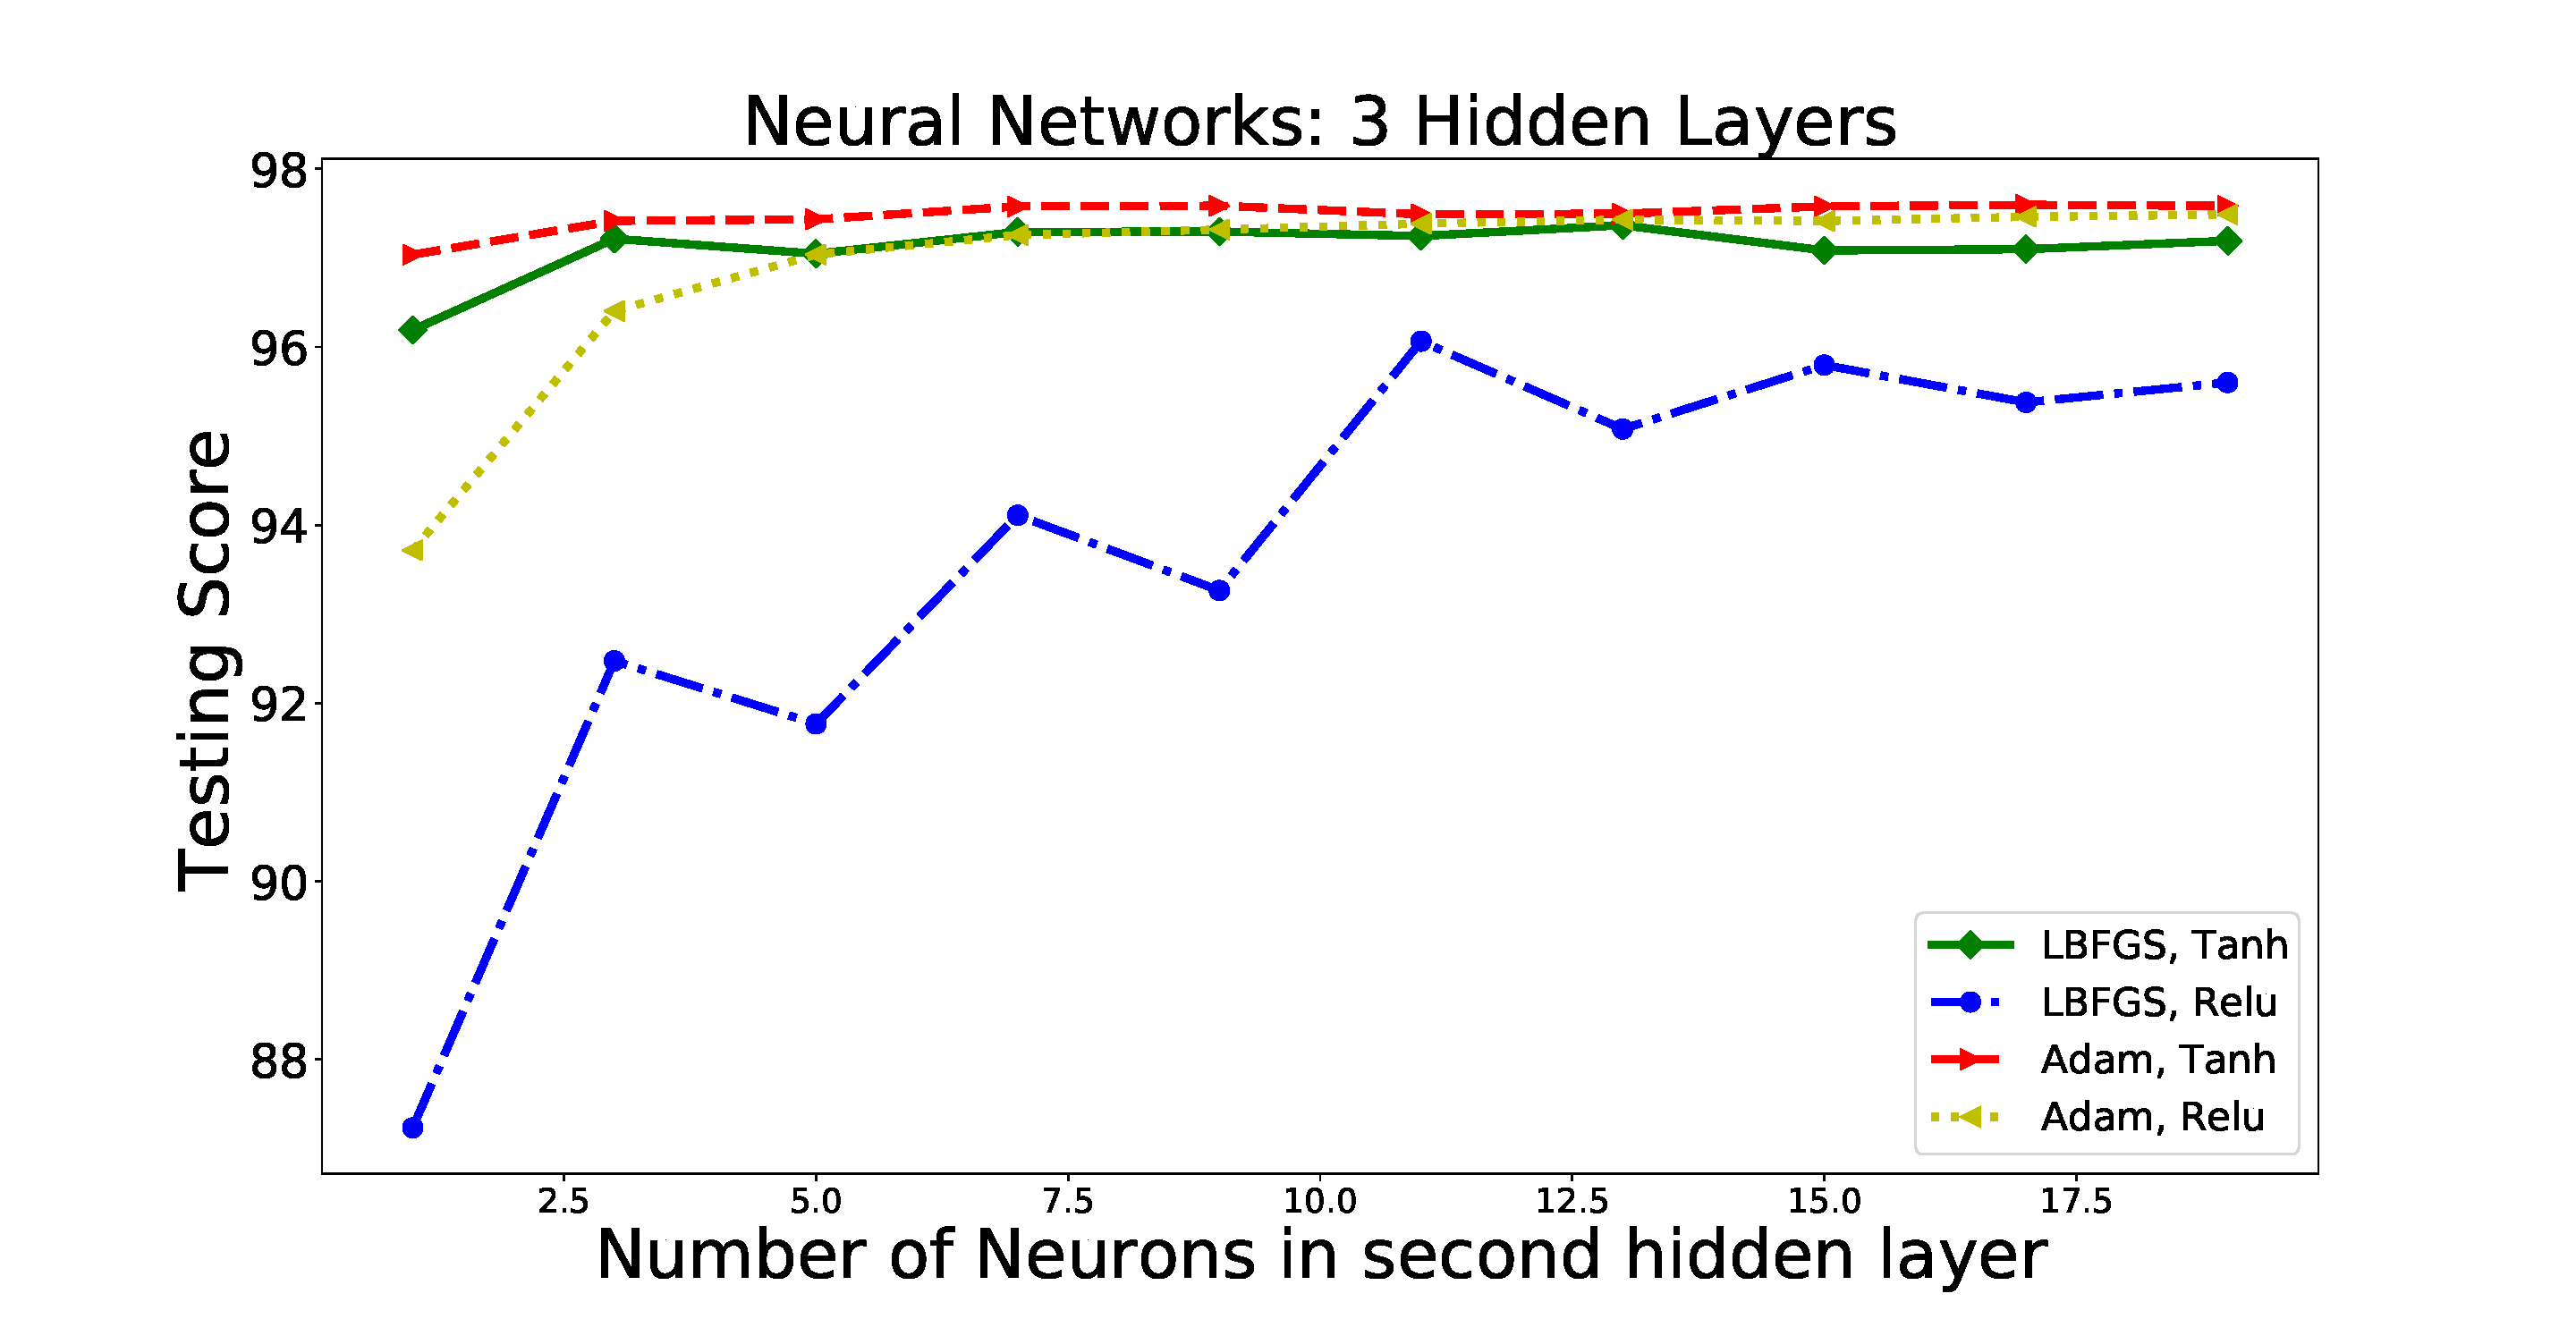
\includegraphics[width=\twopicsp\textwidth]{plots/nn_2layers_3fgl.pdf}
%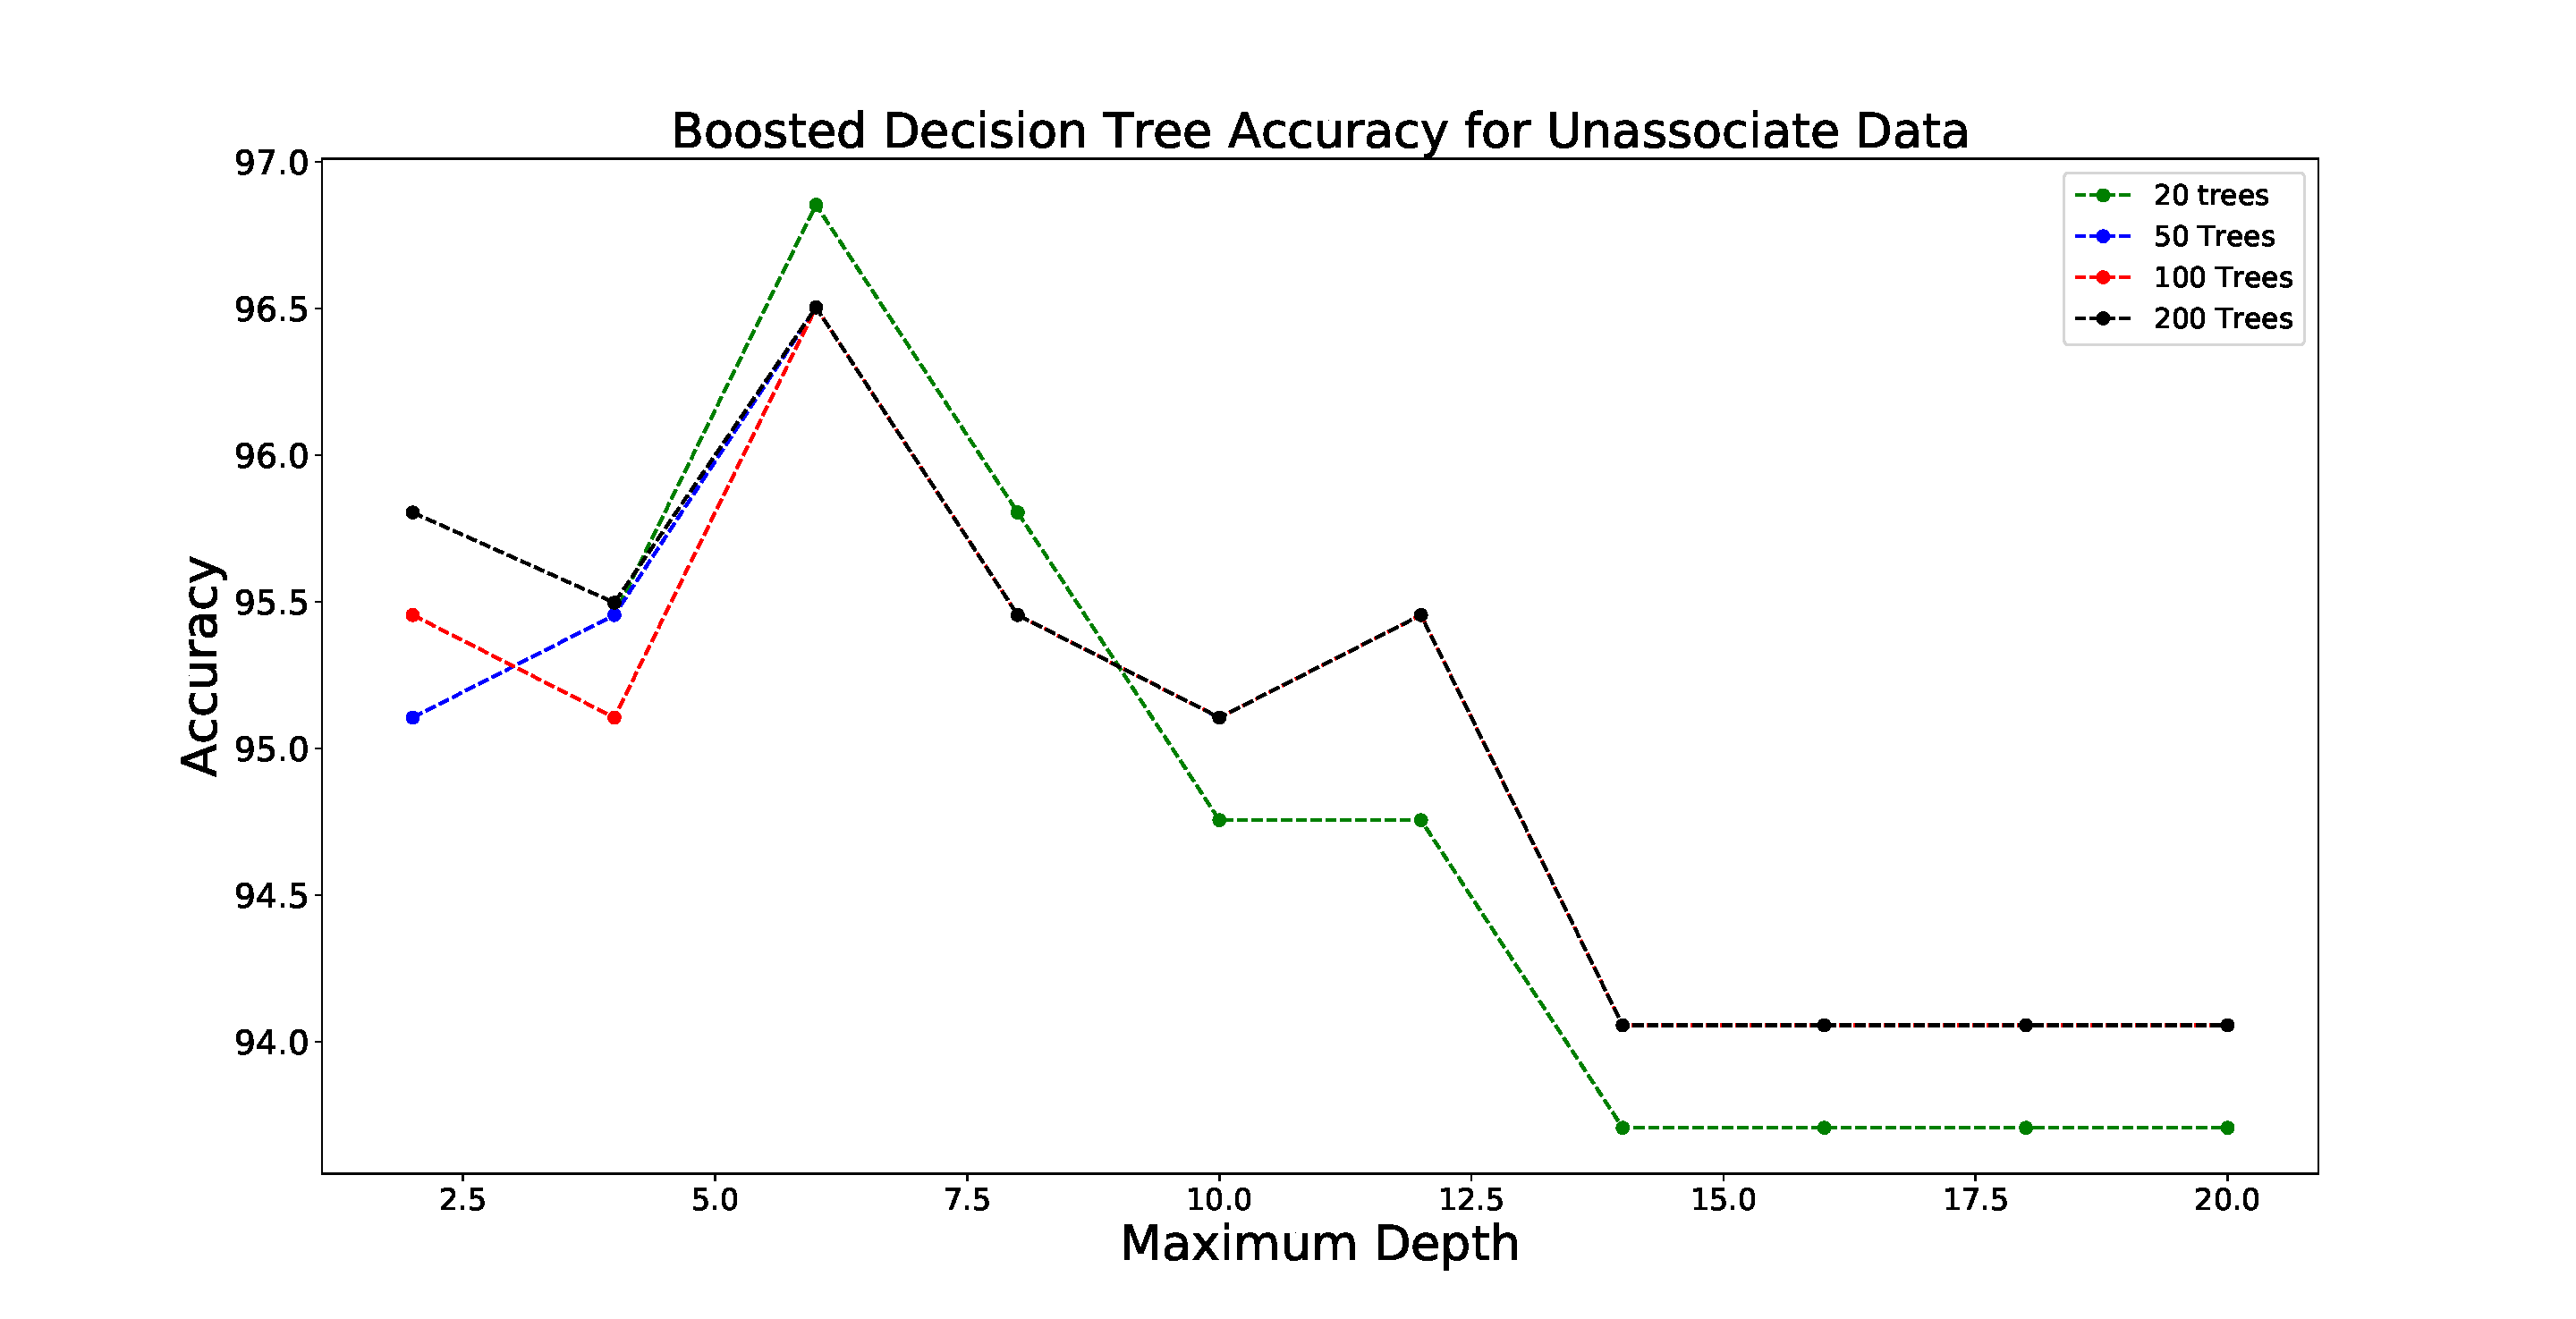
\includegraphics[width=\twopicsp\textwidth]{plots/unassoc_complex.pdf}
\caption{Dependence of NN on the second hidden layer, for 10 neurons in the first layer}
\label{fig:nn_nn}
\end{figure}

%\subsection{Testing on unassociated data}


%Accuracy of the prediction of the source classes compared to the 4FGL classes for RF and BDT algorithms is shown in Figure \ref{fig:RF_BDT_4FGL_accuracy}.



%The accuracy of the RF algorithm increases with the depth of the trees and the number of trees in the forest
%up to maximal depth of about 15 and 200 trees in the forest, after that the accuracy stays constant.
%For the BDT, the accuracy decreases for depth larger than about 10, it does not depend on the number of trees above XXX trees.
%\dima{We should plot BDT with fewer numbers of trees, e.g., 5, 10, 20, 50, it looks like soon after 20 trees BDT converges and accuracy does not change for larger number of trees.}

%Here we can see how Random Forests and BDT accuracies depend on the complexity of the network. Random Forests follow the same pattern as seen with the associated data with greater complexity allowing for a higher accuracy of the sources. Boosted Decision Trees also lower the accuracy as the maximum depth increases, although there seem to be certain points where the accuracy suddenly rises up. As seen with the training data, here also the BDT models converge to an accuracy value which is only dependent on the number of trees\\

%\begin{figure}[h]
%\centerin
%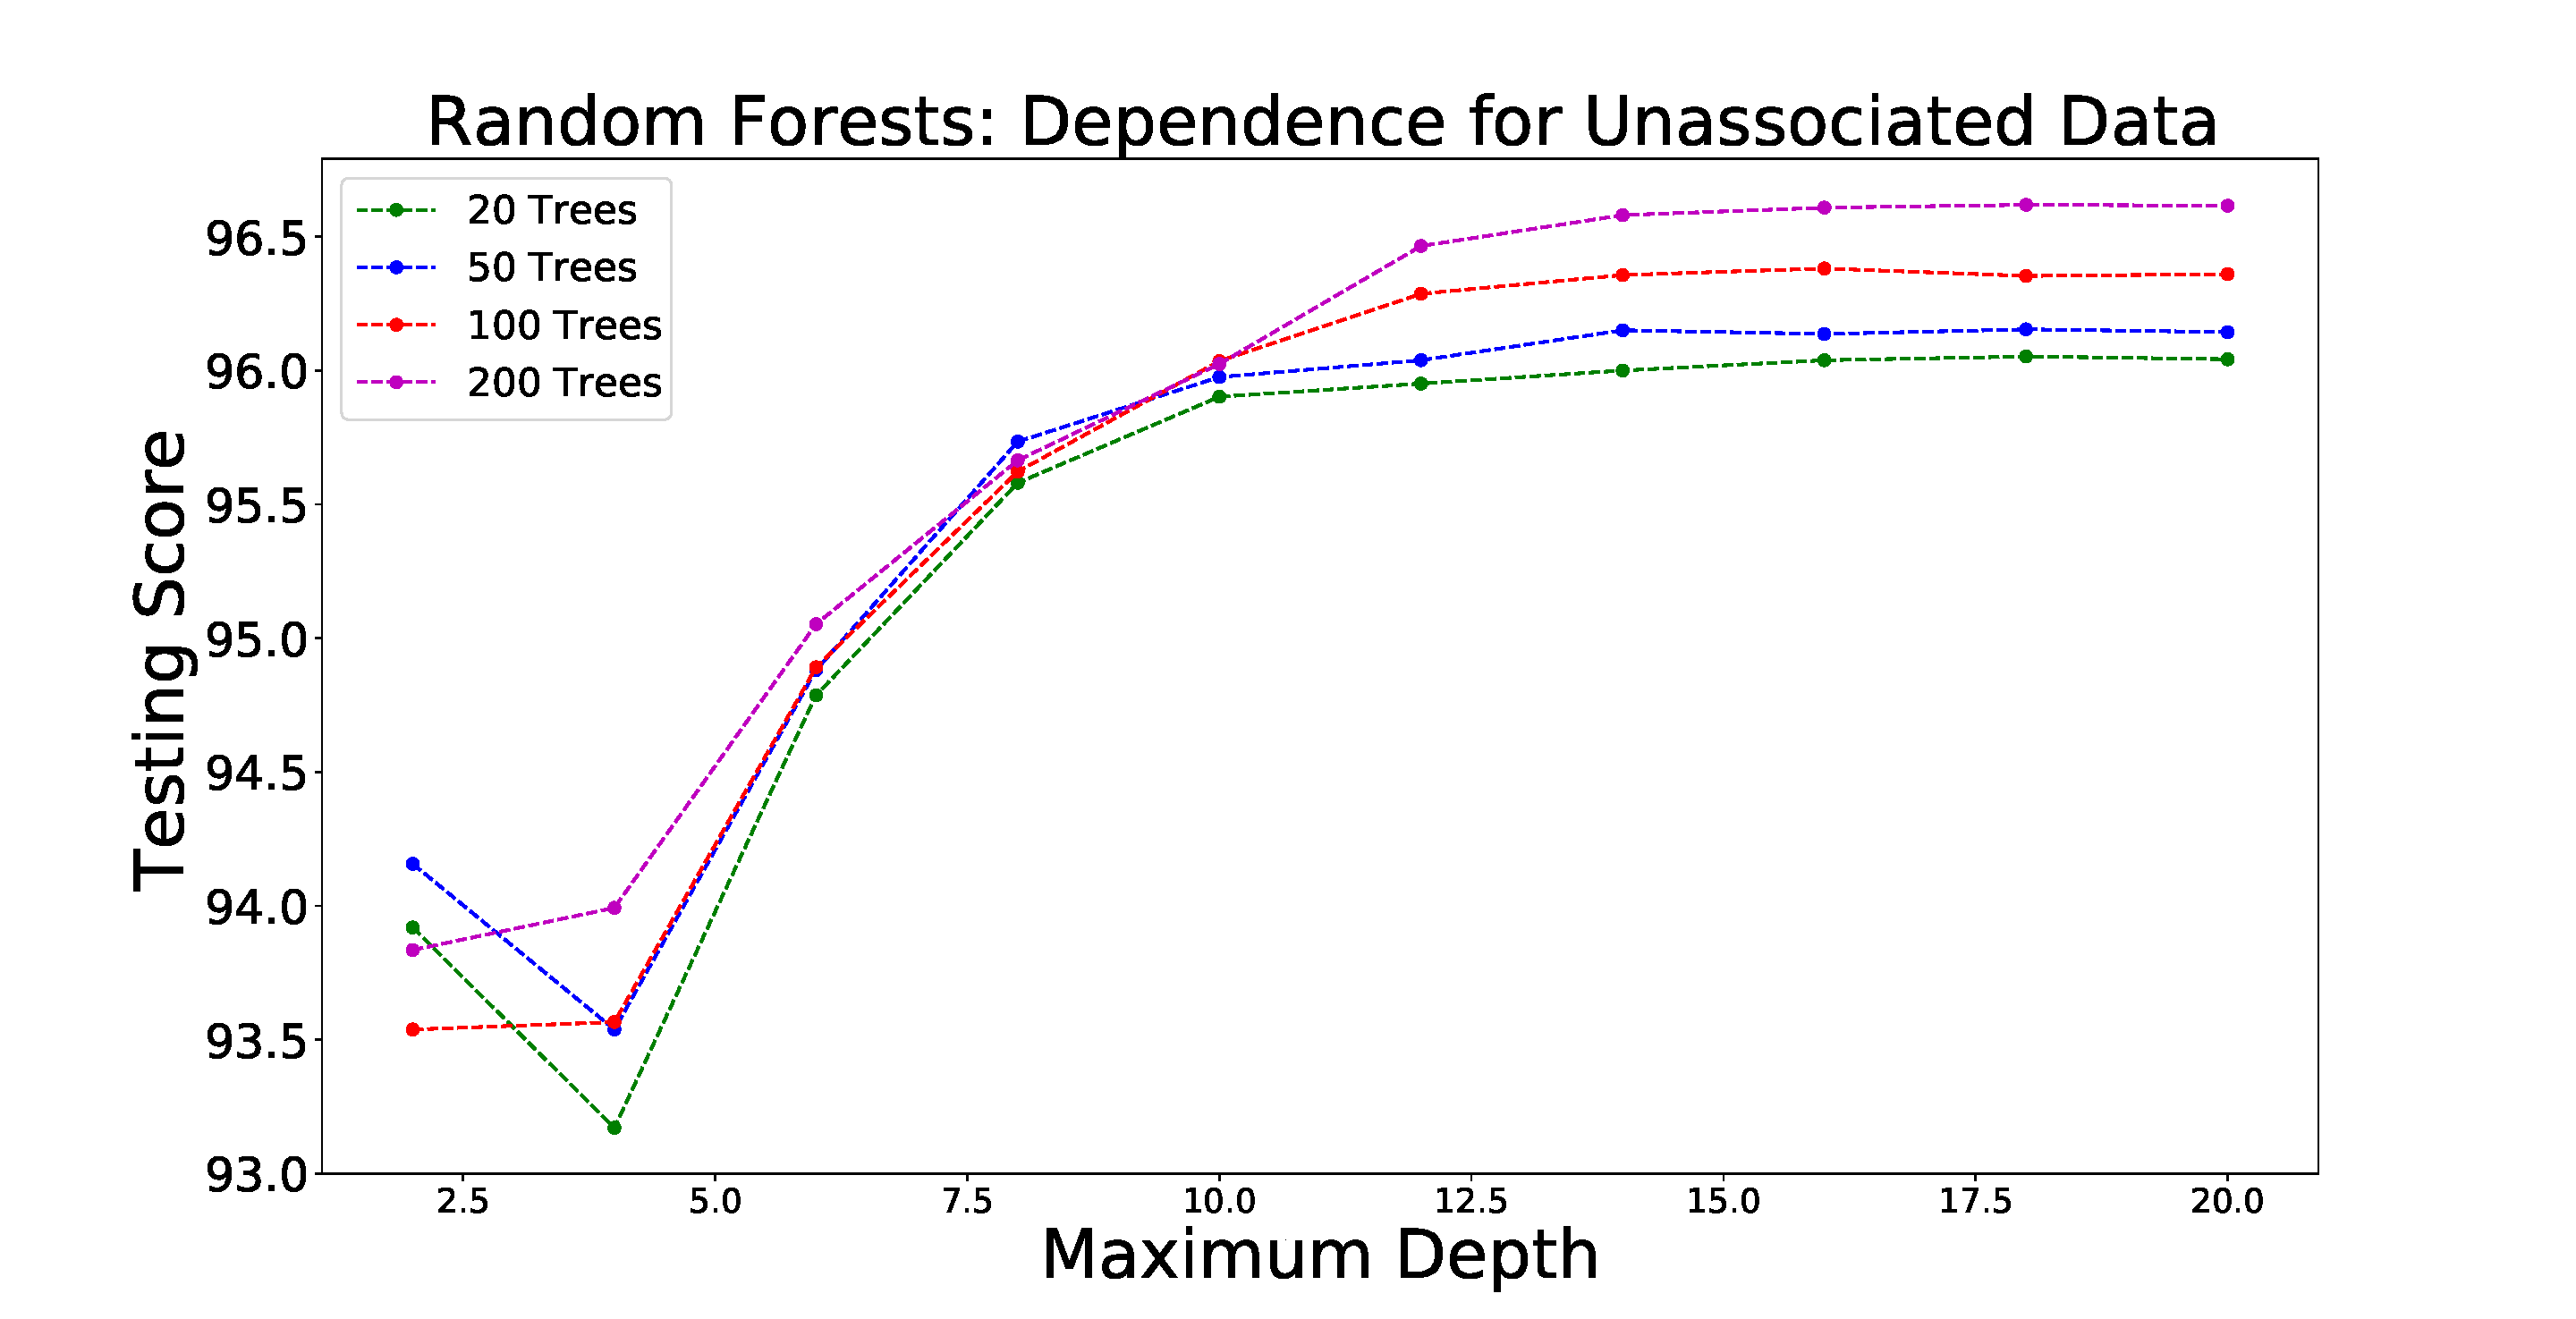
\includegraphics[width=\twopicsp\textwidth]{plots/unassoc2.pdf}
%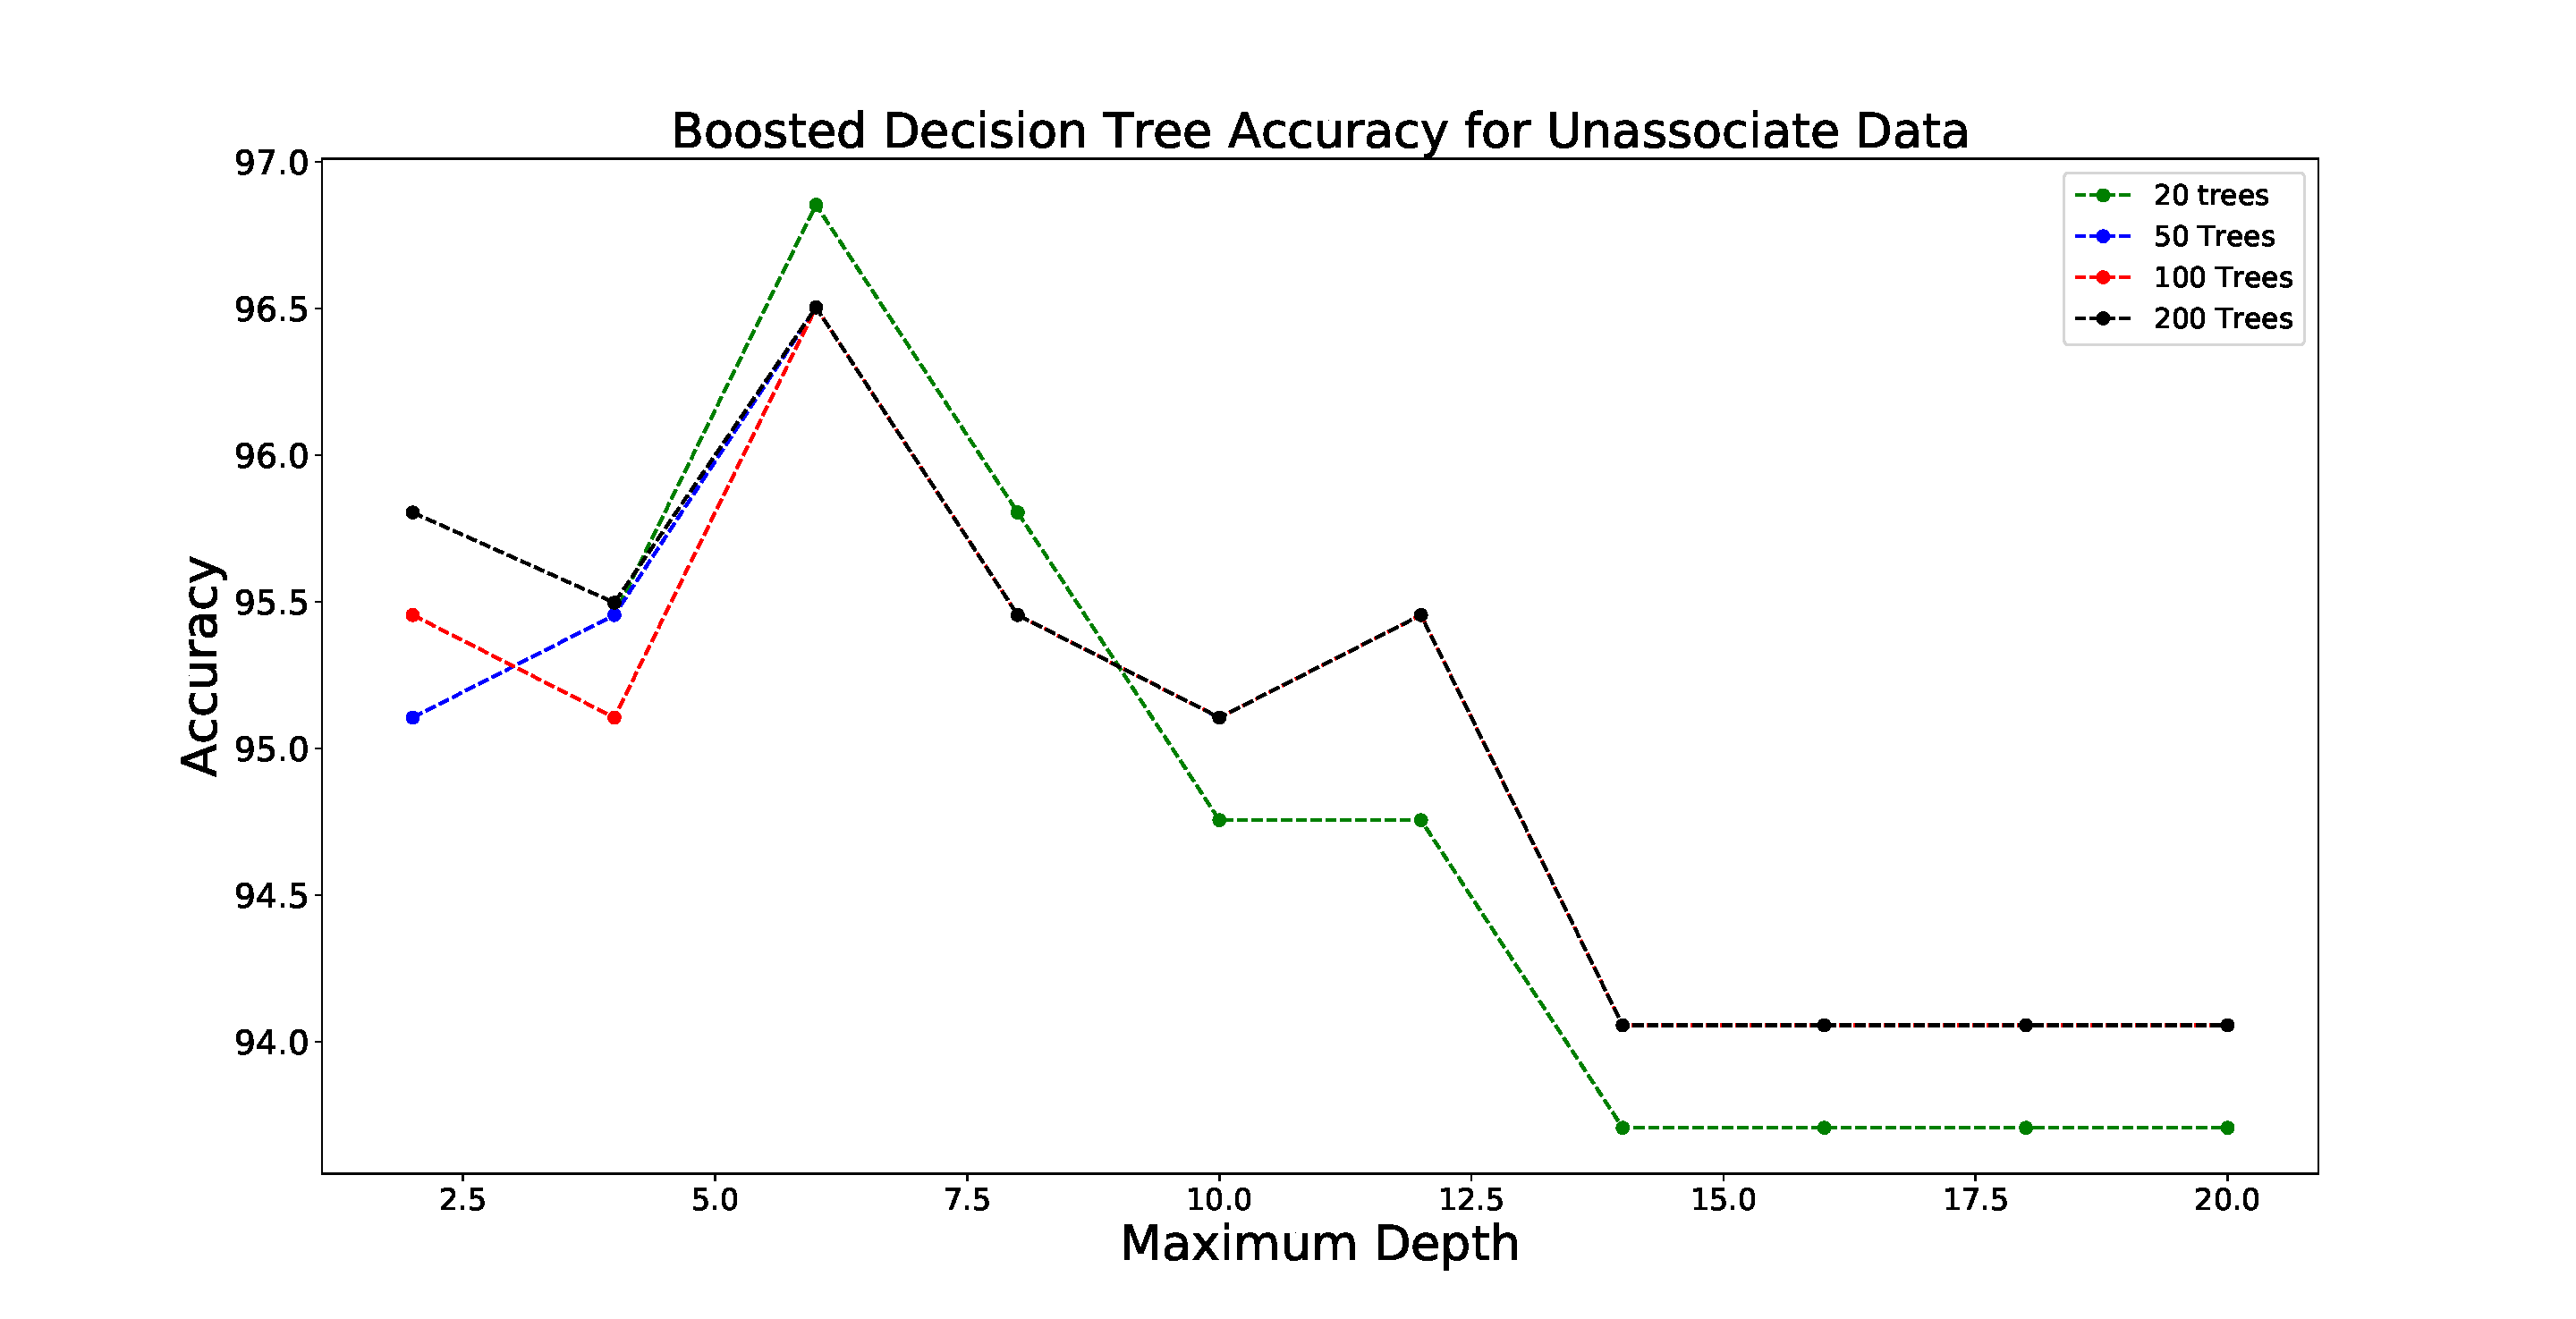
\includegraphics[width=\twopicsp\textwidth]{plots/unassoc_complex.pdf}
%\caption{RF and BDT accuracy of class prediction for unassociated 3FGL sources compared to associations in the 4FGL}
%\label{fig:RF_BDT_4FGL_accuracy}
%\end{figure}

%Neural Networks, unlike random forests are susceptible to overtraining, as can be seen in the figures below. Increase the complexity of the network leads to a slight decrease in accuracy. This is seen for both single hidden layer networks and two hidden layer networks where the first layer has 5 neurons. Here Adam slightly outperforms lbfgs, especially when different activation functions are used. \\
%Accuracies for NN and LR algorithms are presented in Figure \ref{fig:NN_LR_4FGL_accuracy}.
%\dima{As in the previous section, I think we should plot NN for neurons from 2 (or even 1) to about 20, although it really makes sense to plot only up to 10 neurons.}
%An interesting result is found for LR case where the SAGA solver performs better than the L-BFGS, which is different from the results obtained with the training dataset. 
%This is likely because the SAGA solver allows for a more general model than the L-BFGS one. \dima{Why?}

%\begin{figure}[h]
%\centerin
%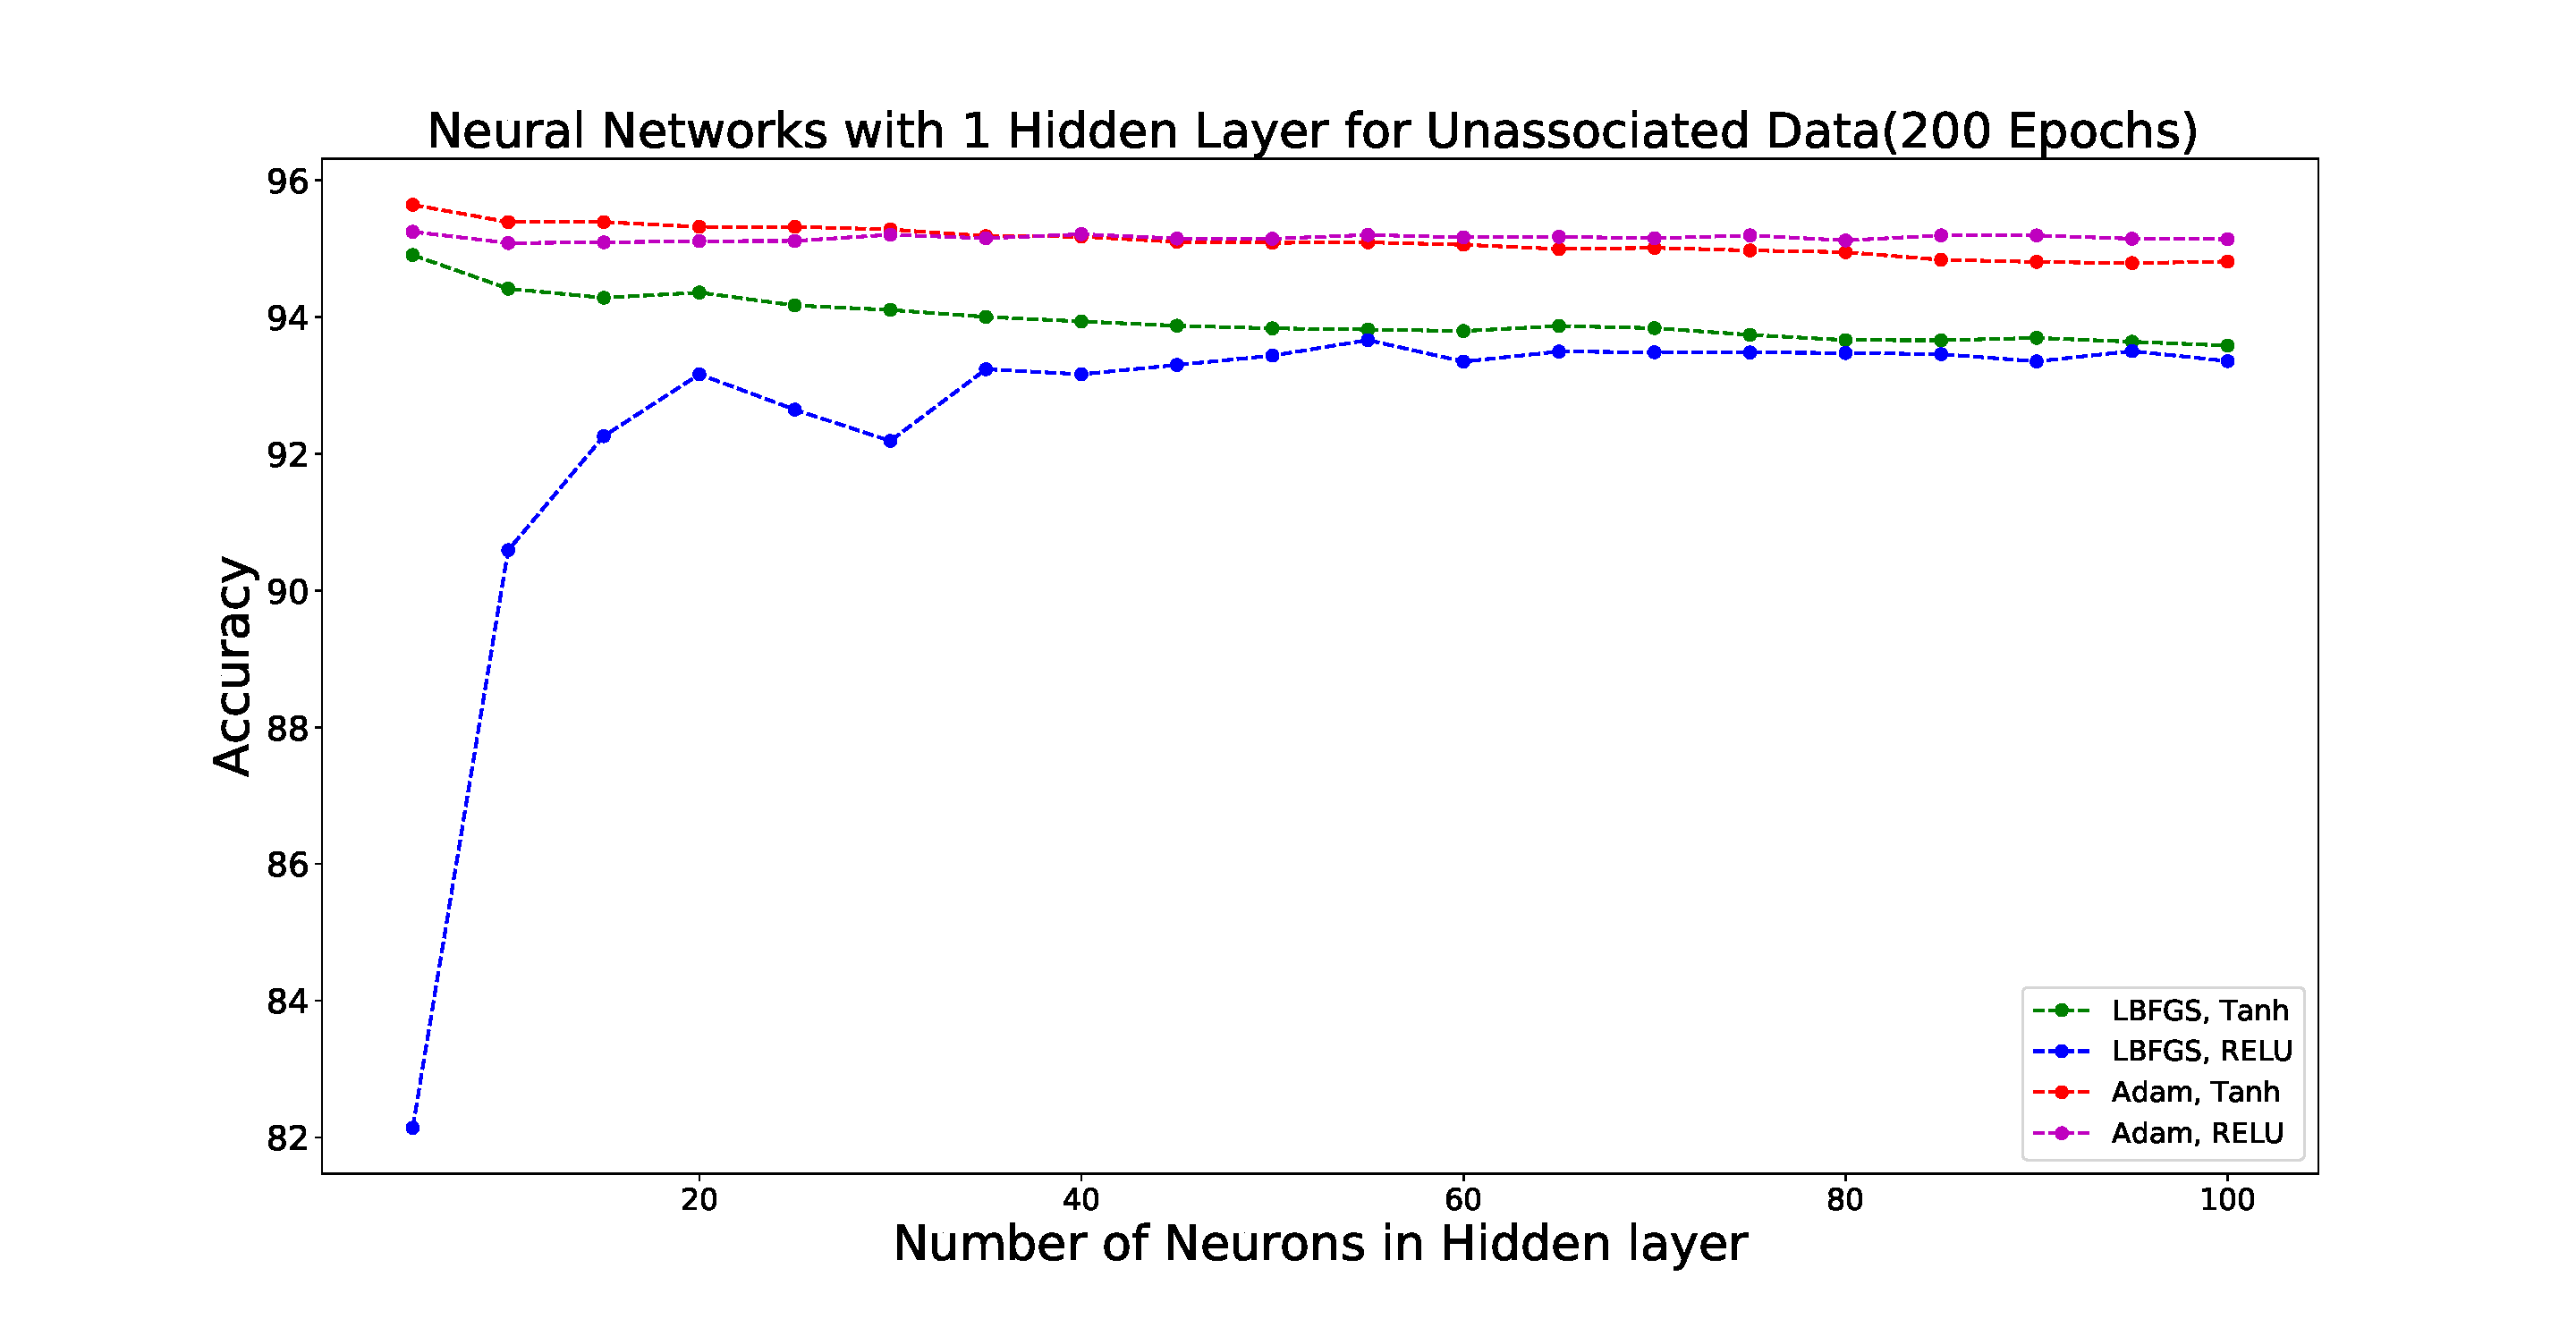
\includegraphics[width=\twopicsp\textwidth]{plots/neurons4.pdf}
%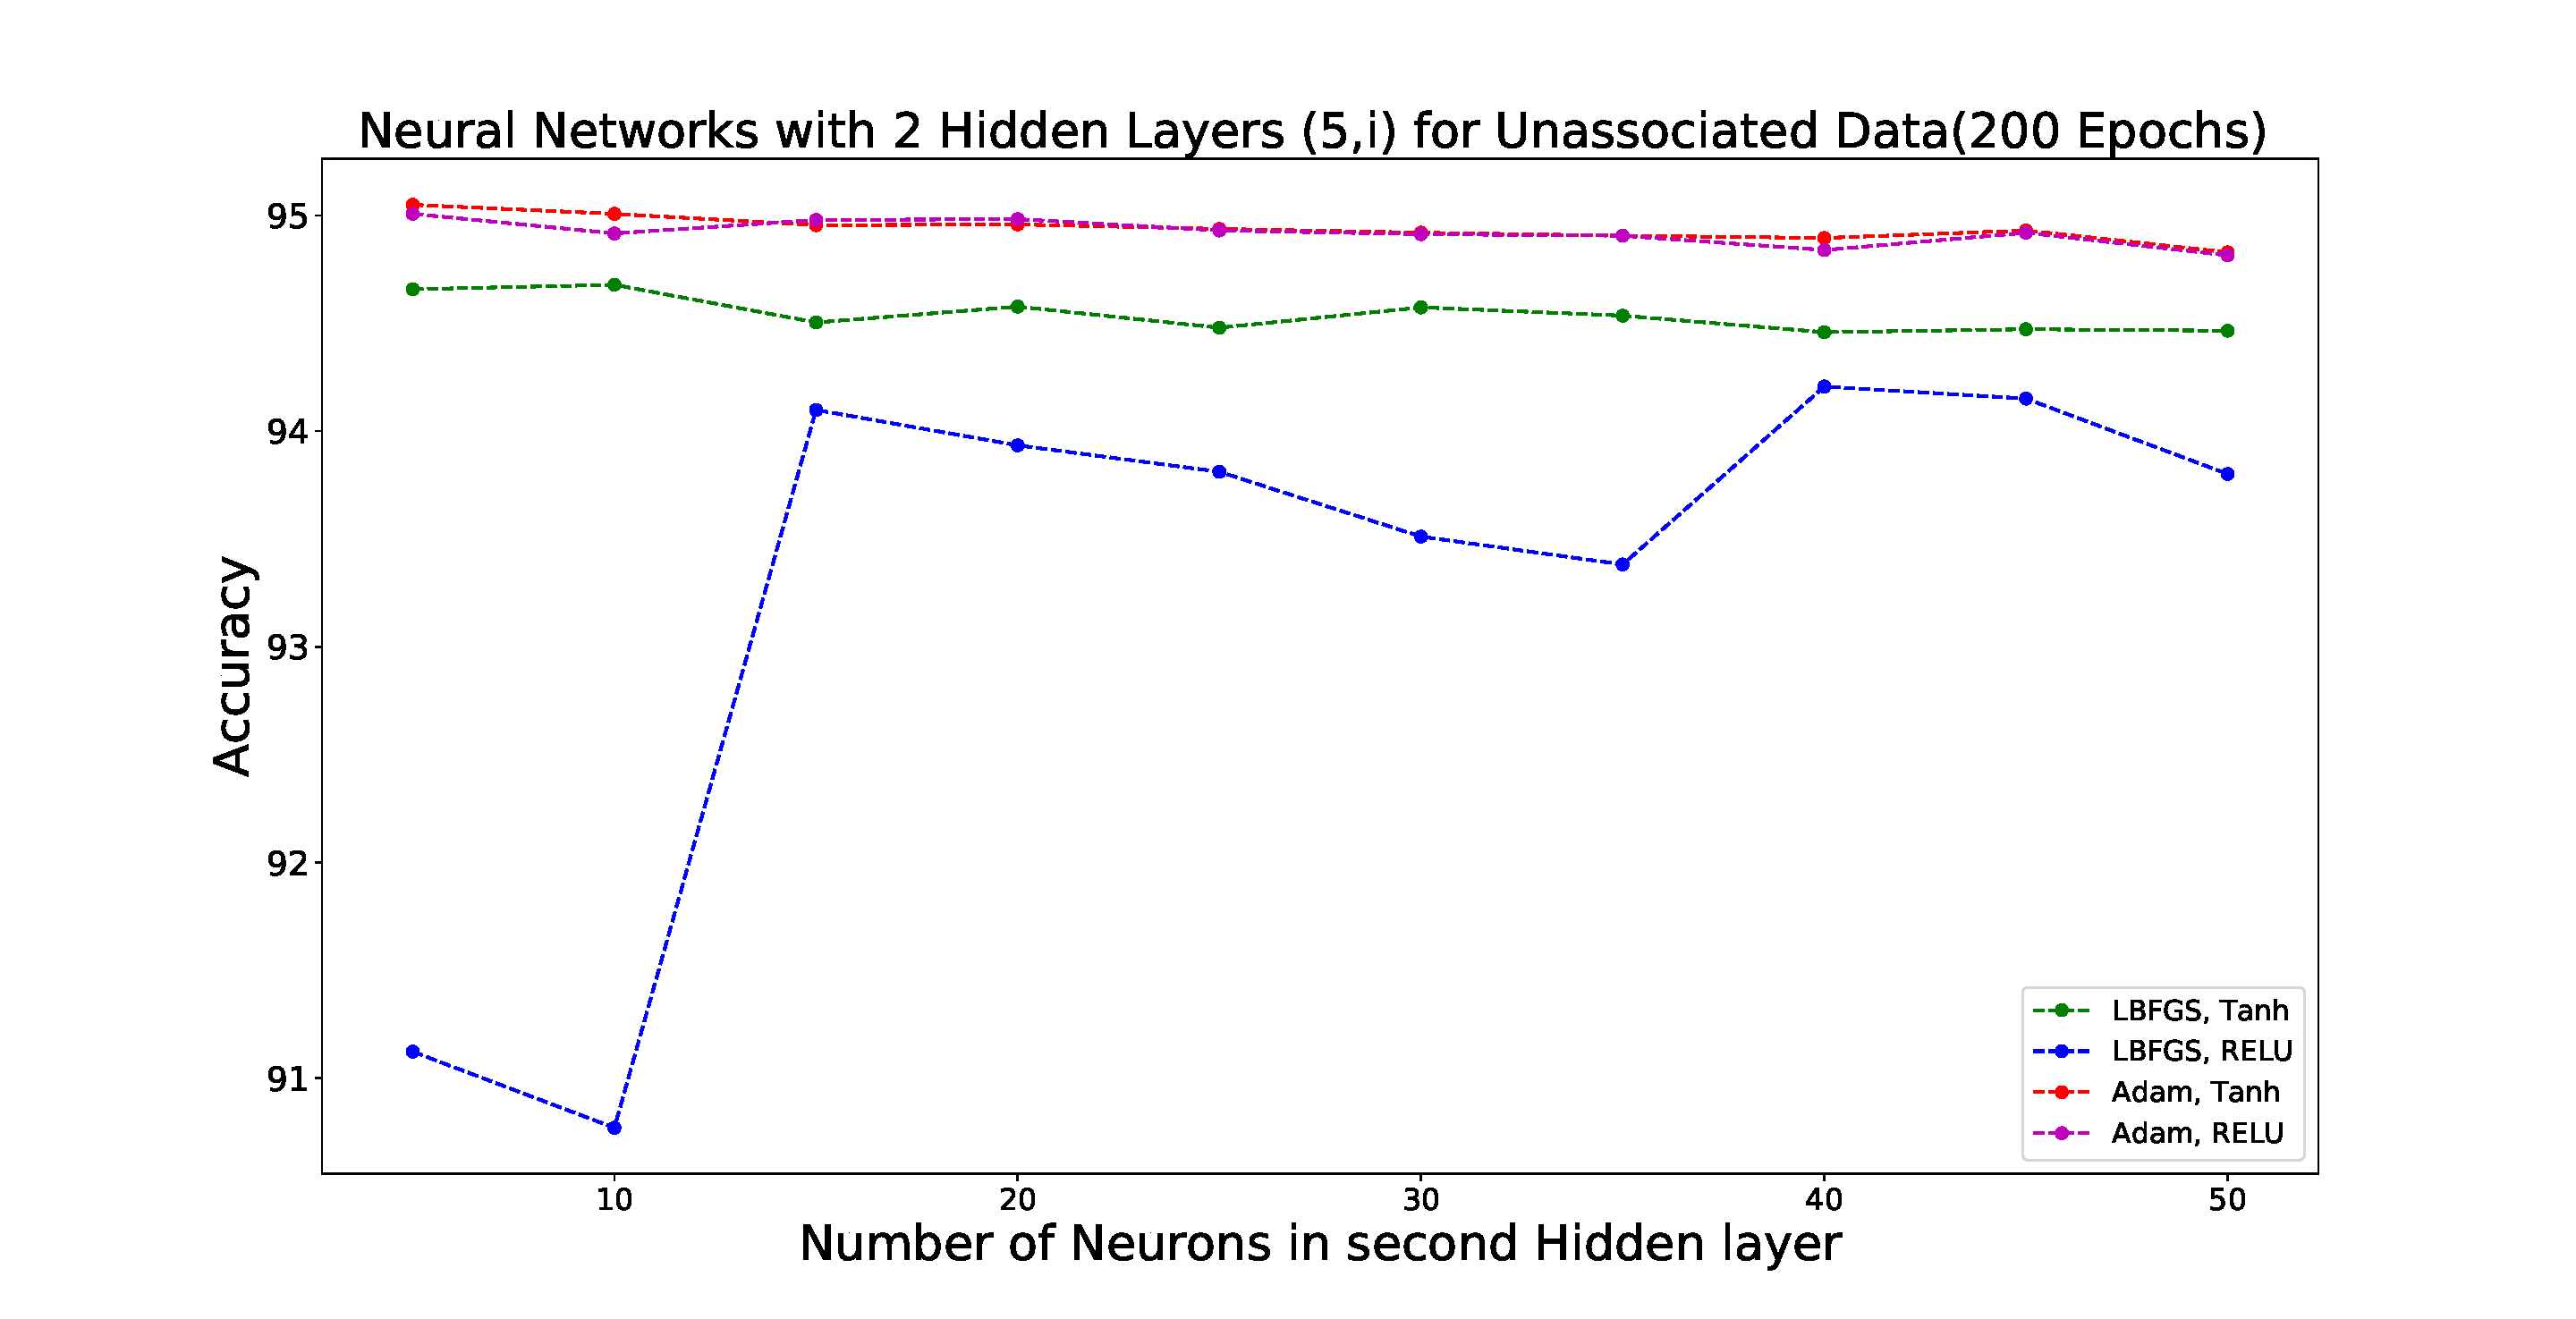
\includegraphics[width=\twopicsp\textwidth]{plots/neurons5.pdf}
%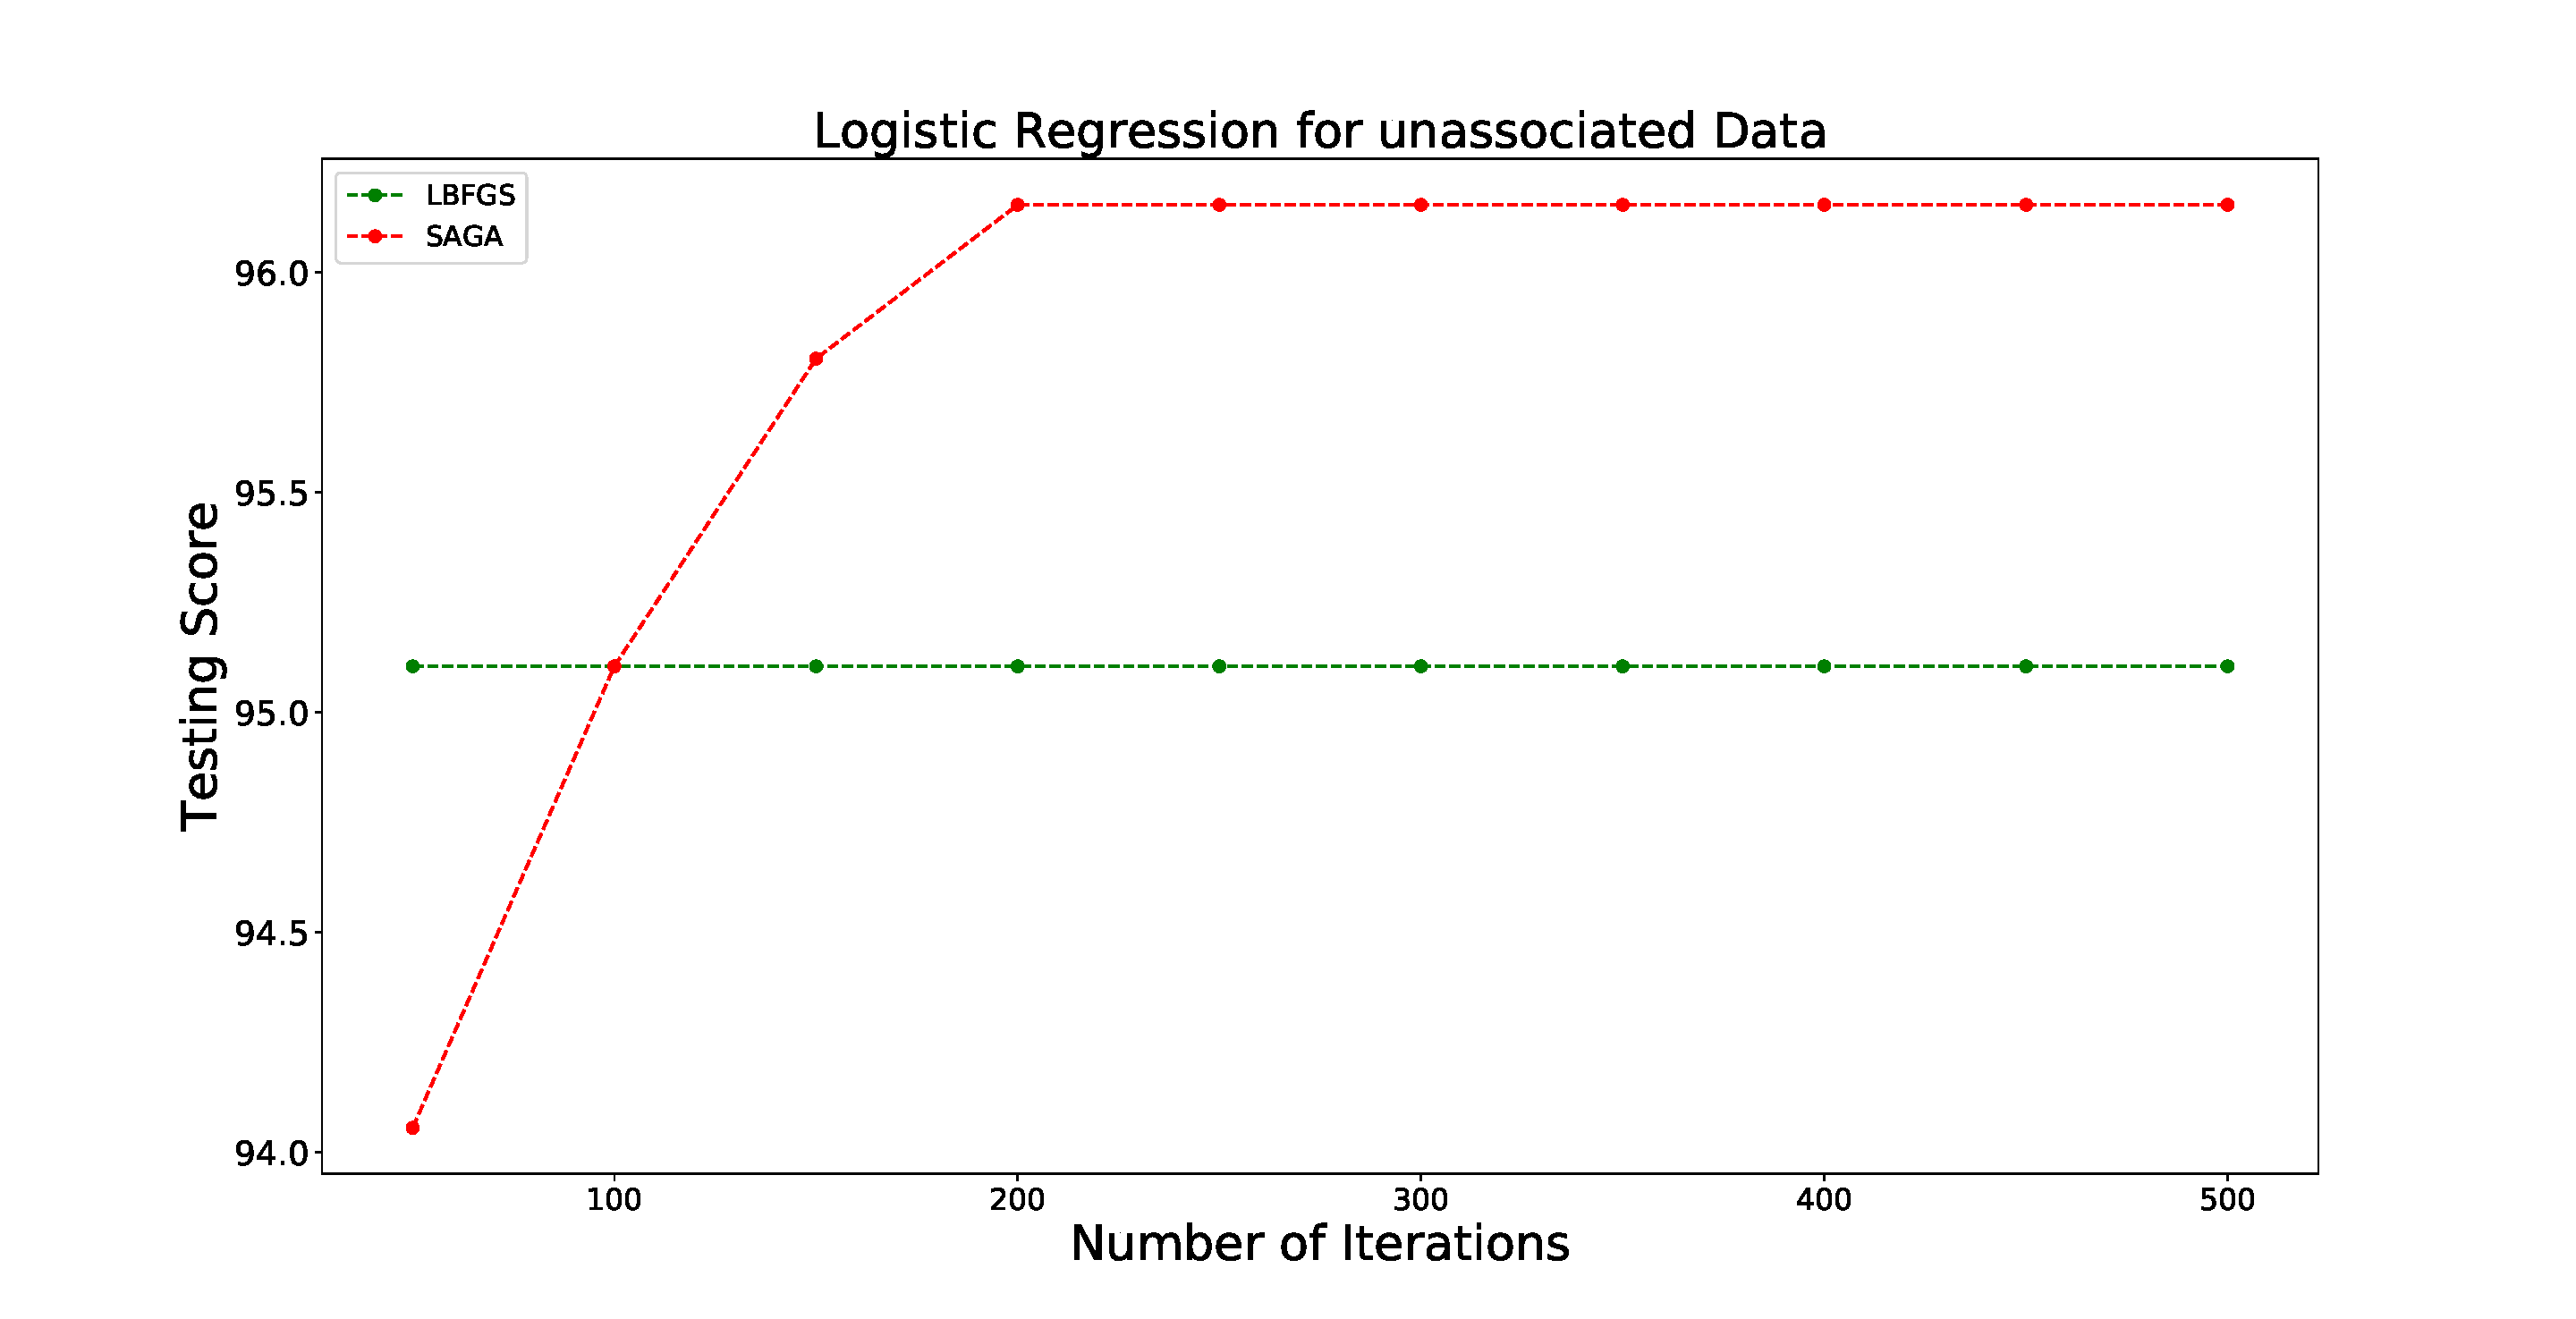
\includegraphics[width=\twopicsp\textwidth]{plots/solver_unass.pdf}
%\caption{Logistic Regression and Neural Network accuracies}
%\label{fig:NN_LR_4FGL_accuracy}
%\end{figure}

